\documentclass[twoside]{amsart}

\usepackage[brazilian]{babel}
\usepackage{csquotes}
%\usepackage[sorting=none, style=verbose-inote, backend=biber]{biblatex}
\usepackage{amsmath}
\usepackage{amssymb}
\usepackage{bbm}
\usepackage{graphics}
\usepackage{mathtools}
\usepackage[hidelinks]{hyperref}
\usepackage{physics}
\usepackage{enumitem}
\usepackage{slashed}
\usepackage[lmargin=0.5cm,rmargin=0.5cm, tmargin =1cm,bmargin =1cm]{geometry}
\usepackage[explicit]{titlesec}
\usepackage{tensor}
\usepackage{cleveref}
\usepackage{ragged2e}
\usepackage{subcaption}

\usepackage{tcolorbox}
\tcbuselibrary{minted,breakable,xparse,skins}

\definecolor{bg}{gray}{0.95}
\DeclareTCBListing{mintedbox}{O{}m!O{}}{%
  breakable=true,
  listing engine=minted,
  listing only,
  minted language=#2,
  minted style=default,
  minted options={%
    linenos,
    gobble=0,
    breaklines=true,
    breakafter=,,
    fontsize=\small,
    numbersep=8pt,
    #1},
  boxsep=0pt,
  left skip=0pt,
  right skip=0pt,
  left=25pt,
  right=0pt,
  top=3pt,
  bottom=3pt,
  arc=5pt,
  leftrule=0pt,
  rightrule=0pt,
  bottomrule=2pt,
  toprule=2pt,
  colback=bg,
  colframe=orange!70,
  enhanced,
  overlay={%
    \begin{tcbclipinterior}
    \fill[orange!20!white] (frame.south west) rectangle ([xshift=20pt]frame.north west);
    \end{tcbclipinterior}},
  #3}

\AtBeginDocument{\renewcommand*{\hbar}{{\mkern-1mu\mathchar'26\mkern-8mu\textnormal{h}}}}
\AtBeginDocument{\newcommand{\e}{\textnormal{e}}}
\AtBeginDocument{\newcommand{\im}{\textnormal{i}}}
\AtBeginDocument{\newcommand{\luz}{\textnormal{c}}}
\AtBeginDocument{\newcommand{\grav}{\textnormal{G}}}
\AtBeginDocument{\newcommand{\kb}{{\textnormal{k}_{\textnormal{B}}}}}
\newcommand{\Dd}[1]{\mathcal D #1}
\newcommand{\trp}[1]{{#1}^{\textnormal{T}}}
\newcommand{\Det}[1]{\textup{Det} #1}

\numberwithin{equation}{section}

\newtheorem{teo}{Teorema}[section]
\newtheorem{defi}{Definição}[section]
\newtheorem{lem}{Lema}[section]
\newtheorem{hip}{Hipótese}[subsection]

\pagestyle{plain}

\titleformat\section[block]
    {\bfseries\centering}
    {\Large Programa \thesection.}
    {\baselineskip}
    {\underbar{#1}}

\titleformat\subsection[block]
    {\bfseries\centering}
    {\Large \thesection.(\Alph{subsection})}
    {\baselineskip}
    {}

%\AddToHook{cmd/section/before}{\clearpage}

%\addbibresource{ref.bib}

\title
{
    \Huge EP1
}
\author
{
    \large Vicente V. Figueira, NUSP: 11809301
}
%\date{\today}

\begin{document}

\maketitle

%\tableofcontents

%%%%%%%%%%%%%%%%%%%%%%%%%%%%%%%%%%%%%%%%%%%%%%%%%%%%%%%%%%%%%

%\begin{refsection}

%\setcounter{section}{1}

\section{\Large Zeros de Funções. Bisseção, Newton-Raphson, Secantes}

\subsection{}

Como requerido pelo enunciado, iremos utilizar do método da Bissecção para 
obter uma solução numérica das raízes da função,

\begin{align}
    f\qty(x) & = x^{\frac34} - \cos\qty(x^2)\label{f}
\end{align}

Conforme o método da Bissecção, escolhemos dois valores iniciais, `$x_0$' 
e `$x_1$', tais que `$x_0<x_1$' e havendo uma raíz contida neste intervalo.
Para a escolha destes valores iniciais, notamos que, cosseno é uma função 
com valor limitado por `$1$', e que a função `$x^{\frac34}$' esta definida 
apenas no intervalo `$\mathbb R^+$' sendo monotônica estritamente 
crescente em seu domínio, sabemos a solução única de 

\begin{align}
    x^{\frac34} = 1\Rightarrow x = 1\nonumber
\end{align}

Sabemos ainda que o primeiro zero da função cosseno em `$\mathbb R^+$' 
ocorre em `$\frac\pi2$', e como `$0<1<\frac\pi2$', segue que,

\begin{align}
    0<\cos\qty(1)<1
\end{align}

Como é verdade também que cosseno é monotônica estritamente decrescente no 
intervalo de `$\qty[0,\frac\pi2]$' segue que também é monotônica 
estritamente decrescente no intervalo de `$\qty[0,1]$' --- Apesar de termos 
analizado para `$\cos\qty(x)$', como `$x^2$' é monotônica estritamente 
crescente no intervalo `$\qty[0,1]$', segue que `$\cos\qty(x^2)$' 
continuará sendo monotônica estritamente decrescente no mesmo intervalo ---. 
Concluimos que,

\begin{itemize}
    \item Se há zeros de `$f\qty(x)$', estes pertencem ao intervalo `$\qty[0,1]$'
    \item `$x^{\frac34}$' é monotônica estritamente crescente no itervalo `$\qty[0,1]$'
    \item `$\cos\qty(x^2)$' é monotônica estritamente decrescente no itervalo `$\qty[0,1]$'
\end{itemize}

Fato de `$\cos\qty(x^2)$' ser decrescente implica que `$-\cos\qty(x^2)$' é 
crescente, logo, `$f\qty(x)$' é a soma de duas funções crescentes, que 
continua sendo uma função crescente,

\begin{itemize}
    \item Se há zeros de `$f\qty(x)$', estes pertencem ao intervalo `$\qty[0,1]$'
    \item `$f\qty(x)$' é monotônica estritamente crescente no itervalo `$\qty[0,1]$'
\end{itemize}

Estes dois fatos por si indicam que se há uma raíz, esta é única, pois para 
haver mais de uma raíz seria necessário que a função trocasse de 
monotonicidade em algum intervalo de seu domínio. 

\begin{itemize}
    \item Se há zeros de `$f\qty(x)$', este é único e pertence ao intervalo `$\qty[0,1]$'
    \item `$f\qty(x)$' é monotônica estritamente crescente no itervalo `$\qty[0,1]$'
\end{itemize}

Para concluírmos sobre a existência do único zero, analizemos o 
comportamento da função sobre a fronteira do intervalo.

\begin{align}
    f\qty(0) = 0^{\frac34} - \cos\qty(0) = -1\nonumber
    f\qty(1) = 1^{\frac34} - \cos\qty(1) = 1-\cos\qty(1)>0\nonumber
\end{align}

Isto é, `$f\qty(0)<0<f\qty(1)$',

\begin{itemize}
    \item Se há zeros de `$f\qty(x)$', este é único e pertence ao intervalo `$\qty[0,1]$'
    \item `$f\qty(x)$' é monotônica estritamente crescente no itervalo `$\qty[0,1]$'
    \item `$f\qty(x)$' troca de sinal no intervalo `$\qty[0,1]$'
\end{itemize}

Para concluir a existência de uma raíz, temos que utilizar de mais uma 
propriedade da função,

\begin{itemize}
    \item Se há zeros de `$f\qty(x)$', este é único e pertence ao intervalo `$\qty[0,1]$'
    \item `$f\qty(x)$' é monotônica estritamente crescente no itervalo `$\qty[0,1]$'
    \item `$f\qty(x)$' troca de sinal no intervalo `$\qty[0,1]$'
    \item `$f\qty(x)$' é contínua no intervalo `$\qty[0,1]$'
\end{itemize}

Os três últimos fatos implicam que a função possui um zero neste intervalo, 
a hipótese da continuidade é crucial, do contrário a função poderia ser 
monotônica estritamente crescente e trocar de sinal via uma discontinuidade 
de tipo salto. Logo somos levados a seguinte conclusão,

\begin{itemize}
    \item `$f\qty(x)$' possui um único zero no intervalo `$\qty[0,1]$'
\end{itemize}

Que pode ser extendida para o maior domínio da função ao notar que 

\begin{align}
    \forall x\in [1,\infty), \ \ x^{\frac34}>\cos\qty(x^2)\Rightarrow \forall x\in [1,\infty),\ \  f\qty(x)>0
\end{align}

Assim, sobre todo o domínio da função concluímos que esta possui apenas 
um zero,

\begin{itemize}
    \item `$f\qty(x)$' possui um único zero em seu domínio `$\mathbb R^+$', sendo este zero contido em `$\qty[0,1]$'
\end{itemize}

Portanto um bom palpite para valores iniciais dos parâmetros é `$x_0=0$' 
e `$x_1=1$'. Para decidir sobre o valor do erro aceitável, nos utilizamos 
de `$10^{-6}$', que se faz uma precisão aceitável do ponto de vista que o 
Python se utiliza por padrão de precisão double que excede este valor de 
casas decimais. A seguir está o código utilizado para rodar o método da Bissecção.

\begin{mintedbox}{python}
import math
import tabulate

#Variáveis necessárias

vPrecisao = 1.E-6

#Função que desejamos encontrar os zeros

def fZero(x): 
    return x**(3/4) - math.cos(x**2)

#Método que adiciona os dados de cada passo em uma tabela

def fTabDados(vIteracao, vInicial, vFinal, vMedio, fZero): 

    tTemp = []
    tTemp.append(vIteracao)
    tTemp.append(vInicial)
    tTemp.append(vFinal)
    tTemp.append(vMedio)
    tTemp.append(fZero(vInicial))
    tTemp.append(fZero(vFinal))
    tTemp.append(vFinal-vInicial)
    
    return tTemp

#Definição do algorítimo do Método da Bissecção

def MetodoBissecao( fZero, #Função da qual queremos encontrar os zeros
                vInicial, #Valor inicial do intervalo
                vFinal): #Valor Final do Intervalo
    
    tDados = [["n","x_0","x_1","x_m","f(x_0)","f(x_1)","Erro"]] #Tabela de Dados

    vIteracao = 0

    #Loop que roda o método até atingir a precisão requerida
    while abs(vInicial - vFinal) > vPrecisao:

        vMedio = (vInicial + vFinal)/2 #Ponto médio do Intervalo

        tDados.append(fTabDados(vIteracao, vInicial, vFinal, vMedio, fZero)) # Dados colocados na tabela

        vIteracao = vIteracao + 1

        if ( (fZero(vInicial) * fZero(vMedio)) > 0 ): #Condicional principal do método
            vInicial = vMedio
        else:
            vFinal = vMedio
    
    tDados.append(fTabDados(vIteracao, vInicial, vFinal, vMedio, fZero))

    return vInicial, tDados

pRaiz, tDados = MetodoBissecao(fZero, 0, 1) #Inicia o método com a função e os valores desejados requeridos

print("A raiz da função é: %.6f" %pRaiz) #Print da Raíz
print()
print(tabulate.tabulate(tDados, headers='firstrow', tablefmt='latex')) #Print dos dados em formato de LaTex
\end{mintedbox}

Utilizando este método foi obtido o seguinte conjunto de dados 
relacionados com a convergência do método.

\centering
{
    \begin{tabular}{rrrrrrr}
        \hline
           $n$ &   $x_0$ &   $x_1$ &   $x_0$ &   $f(x_0)$ &   $f(x_1)$ &        Erro \\
        \hline
           0 &   0        & 1        & 0.5      &  -1           & 0.459698    & 1           \\
           1 &   0.5      & 1        & 0.75     &  -0.374309    & 0.459698    & 0.5         \\
           2 &   0.75     & 1        & 0.875    &  -0.0399971   & 0.459698    & 0.25        \\
           3 &   0.75     & 0.875    & 0.8125   &  -0.0399971   & 0.183754    & 0.125       \\
           4 &   0.75     & 0.8125   & 0.78125  &  -0.0399971   & 0.0658942   & 0.0625      \\
           5 &   0.75     & 0.78125  & 0.765625 &  -0.0399971   & 0.0115372   & 0.03125     \\
           6 &   0.765625 & 0.78125  & 0.773438 &  -0.0145714   & 0.0115372   & 0.015625    \\
           7 &   0.773438 & 0.78125  & 0.777344 &  -0.00160397  & 0.0115372   & 0.0078125   \\
           8 &   0.773438 & 0.777344 & 0.775391 &  -0.00160397  & 0.00494472  & 0.00390625  \\
           9 &   0.773438 & 0.775391 & 0.774414 &  -0.00160397  & 0.00166493  & 0.00195312  \\
          10 &   0.773438 & 0.774414 & 0.773926 &  -0.00160397  & 2.91202e-05 & 0.000976562 \\
          11 &   0.773926 & 0.774414 & 0.77417  &  -0.000787763 & 2.91202e-05 & 0.000488281 \\
          12 &   0.77417  & 0.774414 & 0.774292 &  -0.000379406 & 2.91202e-05 & 0.000244141 \\
          13 &   0.774292 & 0.774414 & 0.774353 &  -0.000175164 & 2.91202e-05 & 0.00012207  \\
          14 &   0.774353 & 0.774414 & 0.774384 &  -7.30273e-05 & 2.91202e-05 & 6.10352e-05 \\
          15 &   0.774384 & 0.774414 & 0.774399 &  -2.19549e-05 & 2.91202e-05 & 3.05176e-05 \\
          16 &   0.774384 & 0.774399 & 0.774391 &  -2.19549e-05 & 3.58229e-06 & 1.52588e-05 \\
          17 &   0.774391 & 0.774399 & 0.774395 &  -9.18639e-06 & 3.58229e-06 & 7.62939e-06 \\
          18 &   0.774395 & 0.774399 & 0.774397 &  -2.80207e-06 & 3.58229e-06 & 3.8147e-06  \\
          19 &   0.774395 & 0.774397 & 0.774396 &  -2.80207e-06 & 3.90105e-07 & 1.90735e-06 \\
          20 &   0.774396 & 0.774397 & 0.774396 &  -1.20599e-06 & 3.90105e-07 & 9.53674e-07 \\
        \hline
        \end{tabular}
}

\justifying
\subsection{}


Agora repetiremos a mesma tarefa de obter a raíz da função, porém, agora utilizando o método de Newton-Raphson, 
para este método necessitamos apenas de um valor inicial como parâmetro, podemos nos utilizar do método anterior 
como um chute para o parâmetro inicial deste método, observando os valores de convergência, podemos tomar `$x_0=0.8$', 
também como neste método a convergência é mais rápida, preferimos aumentar a precisão para `$10^{-10}$', assim o código 
utilizado tomou forma como,

\begin{mintedbox}{python}
import math
import tabulate

#Variáveis necessárias

vPrecisao = 1.E-10

#Função do método de Newton que calcula a próxima aproximação da raíz
def fNewton(x):
    return x - (x**(3/4) - math.cos(x**2))/((3/4)*(x**(-1/4)) + 2*x*math.sin(x**2))

#Função qual desejamos encontrar a raiz
def fZero(x):
    return x**(3/4) - math.cos(x**2)

#Derivada da função que desejamos encontrar a raíz
def fZeroD(x):
    return (3/4)*(x**(-1/4)) + 2*x*math.sin(x**2)

#Função que calcula o erro relativo entre uma aproximação e a próxima aproximação calculada pelo método de Newton
def fErro(x):
    return abs((fNewton(x)-x)/x)

#Método que organiza os dados em tabela
def fTabDados(vIteracao, vInicial, fZero, fErro): 

    tTemp = []
    tTemp.append(vIteracao)
    tTemp.append(vInicial)
    tTemp.append(fZero(vInicial))
    tTemp.append(fZeroD(vInicial))
    tTemp.append(fErro(vInicial))
    
    return tTemp

#Valor inicial da aproximação da raiz
vInicial = 0.8

#Tabela de dados finais
tDados = [["n","x_n","f(x_n)","f'(x_n)","Erro"]]

vIteracao = 0

#Algorítimo do Método de Newton que roda enquanto o erro relativo for maior que a precisão requerida
while fErro(vInicial) > vPrecisao:
    
    tDados.append(fTabDados(vIteracao, vInicial, fZero, fErro))
    
    vIteracao = vIteracao + 1
    vInicial = fNewton(vInicial) #Substitui a aproximação antiga pela próxima calculada pelo método de Newton

tDados.append(fTabDados(vIteracao, vInicial, fZero, fErro))

print("A raiz da função é: %.10f" %vInicial) #Retona a aproximação encontrada para a raiz
print()
print(tabulate.tabulate(tDados, headers='firstrow', tablefmt='latex')) #Retorna a tabela de dados em formato de LaTex
\end{mintedbox}
Com este método podemos ver que a convergência ocorre rapidamente, em apenas `$3$' iterações com um valor de acordo com 
o encontrado pelo método anterior, como pode ser visto pela tabela a seguir,

\centering
\begin{tabular}{rlrrr}
    \hline
       $n$ & $x_n$                &      $f(x_n)$ &   $f'(x_n)$ &        Erro \\
    \hline
       0 & 0.8                & 0.0438013   &   1.74854 & 0.0313127   \\
       1 & 0.7749498302       & 0.000926229 &   1.6752  & 0.000713474 \\
       2 & 0.7743969238       & 4.36101e-07 &   1.67362 & 3.36485e-07 \\
       3 & 0.7743966633 & 9.68114e-14 &   1.67362 & 7.46938e-14 \\
    \hline
\end{tabular}

\justifying

\subsection{}

Neste último item, somos incumbidos de obter a posição de equilíbrio de uma molécula diatômica de NaBr, que pode ser modelada 
com um potencial radial da forma,

\begin{align}
    V\qty(r) = -\frac{\e^2}{4\pi\epsilon_0}\frac1r+V_0\exp\qty(-\frac{r}{r_0})
\end{align}

Para obter a posição de equilíbrio, temos que encontrar uma raiz da força desse sistema, isto é,

\begin{align}
    F\qty(r)= -\dv{V}{r}\qty(r)=-\frac{\e^2}{4\pi\epsilon_0}\frac{1}{r^2}+\frac{V_0}{r_0}\exp\qty(-\frac{r}{r_0})
\end{align}

Vamos resolver este problema dando uma abordagem de quantidades adimensionais, por ser uma abordagem em que podemos utilizar 
o mesmo resultado para outras situações também, para isto vamos nos vantagear de saber as seguintes constantes,

\begin{align}
    K = \frac{\e^2}{4\pi\epsilon_0} = 1.44\cdot 10\ \e\textnormal{V\AA}\\
    V_0 = 1.38\cdot 10^{3}\ \e\textnormal{V}\\
    r_0 = 3.28\cdot 10^{-1}\ \e\textnormal{V}
\end{align}

Para escrever as versões adimensionais do Potencial e da Força, vamos escrever ambas como funções do parâmetro adimensional de 
distância `$x=\frac{r}{r_0}$' de forma que,

\begin{align}
    v\qty(x) = \frac{V\qty(r)}{V_0} = -\frac{K}{V_0r_0}\frac1x+\exp\qty(-x)\\
    f\qty(x) = \frac{r_0}{V_0}F\qty(r) = -\frac{K}{V_0r_0}\frac{1}{x^2}+\exp\qty(-x)
\end{align}

Com o valor constante adimensional

\begin{align}
    \frac{K}{V_0r_0} &=\frac{1.44}{3.28\cdot1.38}10^{-1}
\end{align}

O gráfico de ambas as funções pode ser visto abaixo,

\begin{figure}[h]
    \begin{subfigure}{0.4\textwidth}
        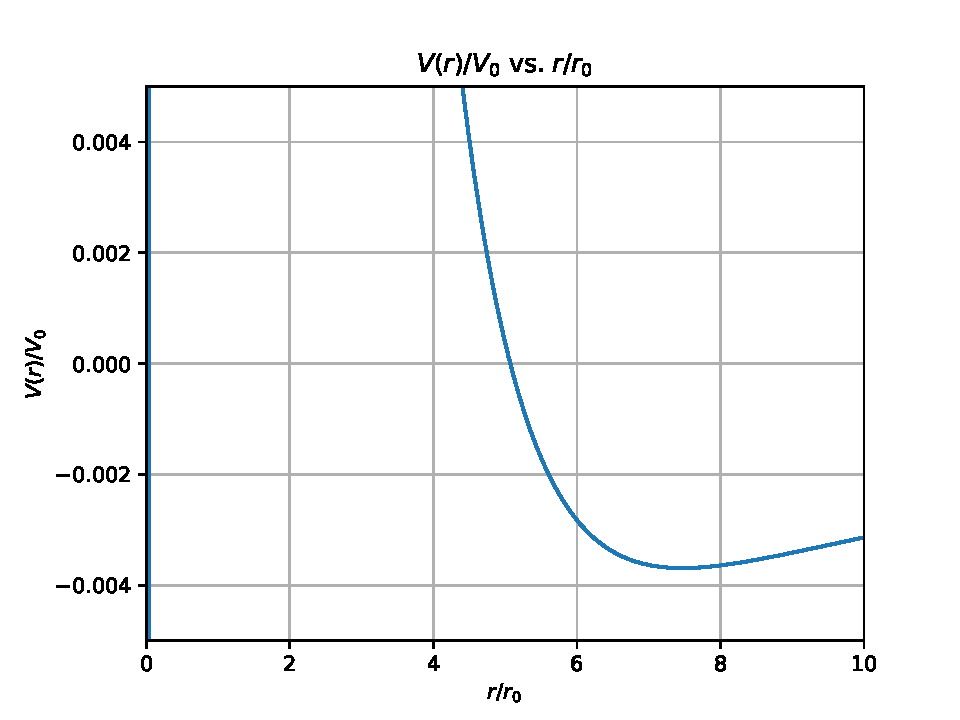
\includegraphics[width=1\linewidth, height=6cm]{potencial.pdf}
    \end{subfigure}
    \begin{subfigure}{0.4\textwidth}
        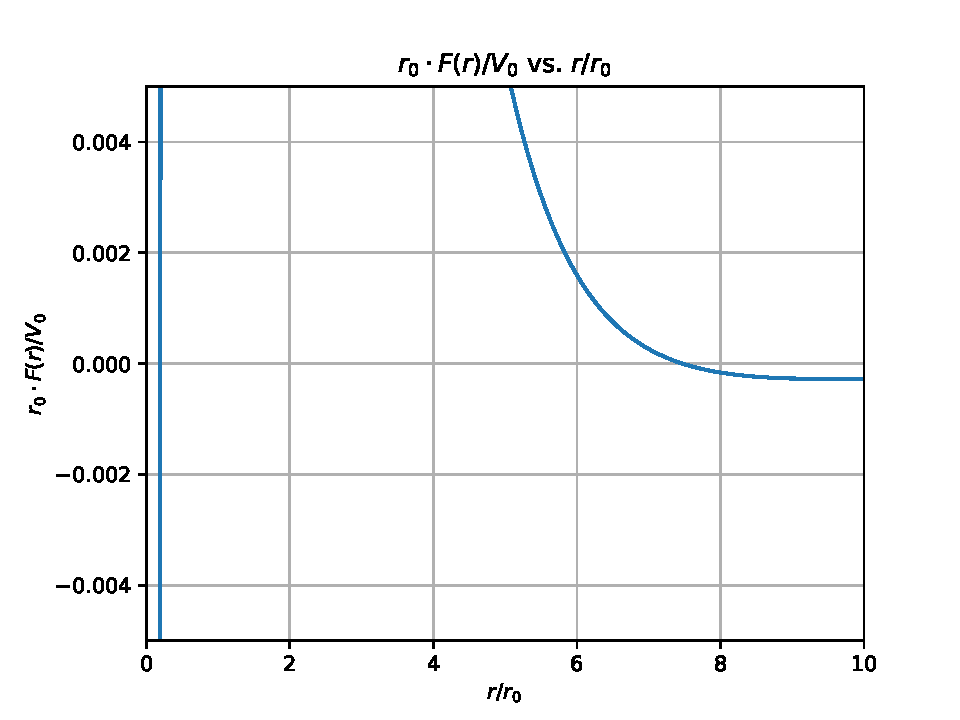
\includegraphics[width=1\linewidth, height=6cm]{forca.pdf}
    \end{subfigure}
\end{figure}

Nestes gráficos podemos ver claramente que há um mínimo do potencial entre `$x=6$' e `$x=8$' e que a força possui 
uma raiz entre `$x=6$' e `$x=8$'. O que nos permite fazer um chute para os dois parâmetros iniciais necessários para 
o método da secante, para os quais utilizamos os valores de `$x_0=6$' e `$x_1=6.5$', a precisão desejada foi fixada como 
`$10^{-10}$' pois também este método converge rapidamente, o código utilizado pode ser visto abaixo,

\begin{mintedbox}{python}
import math
import tabulate

#Constantes Físicas utilizadas

vV_0 = 1.38E3 # eV
vR_0 = 3.28E-1 # Angstrom
vK = 1.44E1 # eV * Angstrom

#Variáveis necessárias

vPrecisao = 1E-10

#Função Potencial
def fPotencial(x):
    return -(vK/(vV_0*vR_0))/x+math.exp(-x)

#Função Força
def fForca(x):
    return -(vK/(vV_0*vR_0))/(x**2)+math.exp(-x)

#Método Secante que retorna a próxima aproximação partindo de dois pontos de aproximação
def fSecante(vInicial, vFinal):
    return vFinal - fForca(vFinal)*(vFinal - vInicial)/(fForca(vFinal) - fForca(vInicial))

#Função que retorna o erro relativo do segundo ponto de aproximação com a próxima correção calculada pelo método das secantes
def fErro(vInicial, vFinal):
    return abs((fSecante(vInicial, vFinal) - vFinal)/vFinal)

#Método para salvar dados em tabelas
def fTabDados(vIteracao, vInicial, vSegundo, fSecante, fForca, fErro): 

    tTemp = []
    tTemp.append(vIteracao)
    tTemp.append(vInicial)
    tTemp.append(vSegundo)
    tTemp.append(fSecante(vInicial, vSegundo))
    tTemp.append(fForca(vSegundo))
    tTemp.append(fForca(fSecante(vInicial, vSegundo)))
    tTemp.append(fErro(vInicial, vSegundo))

    return tTemp

#Valores iniciais para os dois parâmetros de aproximação necessitados pelo método das secantes
vInicial = 6
vSegundo = 6.5

tDados = [["n","x_{n-1}","x_{n}", "x_{n+1}","f(x_n)","f(x_{n+1})","Erro"]]

vIteracao = 0

#Loop principal do método que roda enquanto o erro entre a próxima correção for menor que a precisão requisitada
while fErro(vInicial, vSegundo) > vPrecisao:

    #Adiciona dados na tabela
    tDados.append(fTabDados(vIteracao, vInicial, vSegundo, fSecante, fForca, fErro))

    vIteracao = vIteracao + 1

    #Algorítimo do Método das secantes
    vTemp = fSecante(vInicial, vSegundo) #Variável temporária que guarda o valor da próxima aproximação
    vInicial = vSegundo #Transfere o valor da segunda aproximação para a primeira
    vSegundo = vTemp #Transfere para a segunda aproximação a nova aproximação gerada pelo método

tDados.append(fTabDados(vIteracao, vInicial, vSegundo, fSecante, fForca, fErro))

print("O raio de equilíbrio é r_eq/r_0 = %.10f" %vSegundo) #Print da aproximação final
print()
print(tabulate.tabulate(tDados, headers='firstrow', tablefmt='latex')) #Print dos dados de cada iteração como forma de Tabela para LaTex
\end{mintedbox}

Utilizando este código foi obtido as seguintes aproximações,

\centering
\begin{tabular}{rlllrrr}
    \hline
       $n$ & $x_{n-1}$            & $x_{n}$              & $x_{n+1}$            &      $f(x_n)$ &   $f(x_{n+1})$ &        Erro \\
    \hline
       0 & 6            & 6.5          & 6.9442761991 & 0.00075046  &  0.000304424 & 0.0683502   \\
       1 & 6.5          & 6.9442761991 & 7.2474991215 & 0.000304424 &  0.000106287 & 0.0436652   \\
       2 & 6.9442761991 & 7.2474991215 & 7.4101566299 & 0.000106287 &  2.57075e-05 & 0.0224433   \\
       3 & 7.2474991215 & 7.4101566299 & 7.4620500379 & 2.57075e-05 &  3.13908e-06 & 0.00700301  \\
       4 & 7.4101566299 & 7.4620500379 & 7.4692679732 & 3.13908e-06 &  1.11164e-07 & 0.000967286 \\
       5 & 7.4620500379 & 7.4692679732 & 7.4695329653 & 1.11164e-07 &  5.05909e-10 & 3.54776e-05 \\
       6 & 7.4692679732 & 7.4695329653 & 7.4695341768 & 5.05909e-10 &  8.20651e-14 & 1.62192e-07 \\
       7 & 7.4695329653 & 7.4695341768 & 7.4695341770 & 8.20651e-14 & -1.0842e-19  & 2.6314e-11  \\
    \hline
\end{tabular}

\justifying

Aqui deve ser levado em conta que foi calculado a posição de equilíbrio adimensional, que no caso é, `$x=\frac{r}{r_0}$', 
para obter o valor em Angstrom, basta tomar,

\begin{align}
    r_{eq}=x_{eq}r_0=7.4695341770\cdot3.28\cdot10^{-1}\textnormal{\AA}=2.4500072101\textnormal{\AA}
\end{align}

O erro calculado continua sendo o mesmo, pois este foi calculado como erro relativo, que de qualquer forma é adimensional, 
não sendo alterado por multiplicar a variável de interesse por uma constante


\end{document}